\chapter{Dealing with geographical variation: hepatitis C}
\label{applications-rfx}

One challenge in global disease modeling for descriptive
epidemiological estimation is properly reflecting the true regional
variation in disease epidemiology. While some diseases are relatively
consistent in their levels and age patterns from region to region,
others vary a great deal.  The most extreme examples of this are focal
diseases which are only present in certain regions, but the hardest to
model are diseases that are present globally, but to greater and lesser
degree.  Hepatitis C Virus (HCV) is an example of such a disease,
which we examine in this chapter.  In the absence of any strongly
predictive covariates, we use hierarchical random effects to model
this regional variation.

Hepatitis C is a viral infection that attacks the liver.  In a small
portion of acute cases, the body can eliminate the virus; however the
majority of acute cases develop into chronic infections.  Chronic
infections cause liver damage and may develop into end stage liver
disease or cirrhosis.  Few, if any, chronic cases experience symptoms
and only one third of acute cases are symptomatic and jaundice.
Chronic symptoms are nonspecific, intermittent and mild with the most
common symptom being fatigue.  Common symptoms for severe and advanced
disease stages include nausea, dark urine and jaundice.  Since
hepatitis C infections are asymptomatic, diagnosis requires laboratory
testing for both hepatitis antibodies (anti-HCV) and the hepatitis
virus (HCV RNA).  There is no vaccination for hepatitis C, but therapy
can prevent advanced liver disease. \cite{hoofnagle_hepatitis_1997,
  ghany_diagnosis_2009}

Compared to other countries in the North Africa/Middle East region,
Egypt has a high hepatitis C prevalence.  In an attempt to treat
endemic schistosomiasis, a common parasitic worm that affects the
urinary tract, gut and liver, the Egyptian Ministry of Health launched
widespread injection-based treatment throughout 1950-1980.  While
there were improvements in schistosomiasis-induced mortality, recycled
needles and poor needle sterilization infected many with hepatitis
C. \cite{frank_role_2000, mezban_hepatitis_2006,
  strickland_liver_2006} The spatial variations of hepatitis C in
North Africa and the Middle East provides a striking example for
hierarchical random effects modeling.

Random effects modeling detects systematic differences among different
hierarchies, or levels, of data.  The spatial hierarchy in the GBD
2010 study uses countries nested in regions nested in super-regions.
There are $21$ regions defined by demographic and epidemiological
similarities that are further clustered by $7$ super-regions.

The analysis of hepatitis C infection uses data on the prevalence of persons who
have hepatitis C antibodies.  Incomplete data or data from high-risk
populations, such as health care workers, were excluded.
Figure~\ref{fig:app-hepc data} shows data collected in systematic
review for two countries in the North Africa/Middle East region, Egypt
and Jordan.  Notice that for some age groups, hepatitis C prevalence
measurements in Egypt are more than $40$ times higher the corresponding measurements in
Jordan.

    \begin{figure}[h]
        \begin{center}
            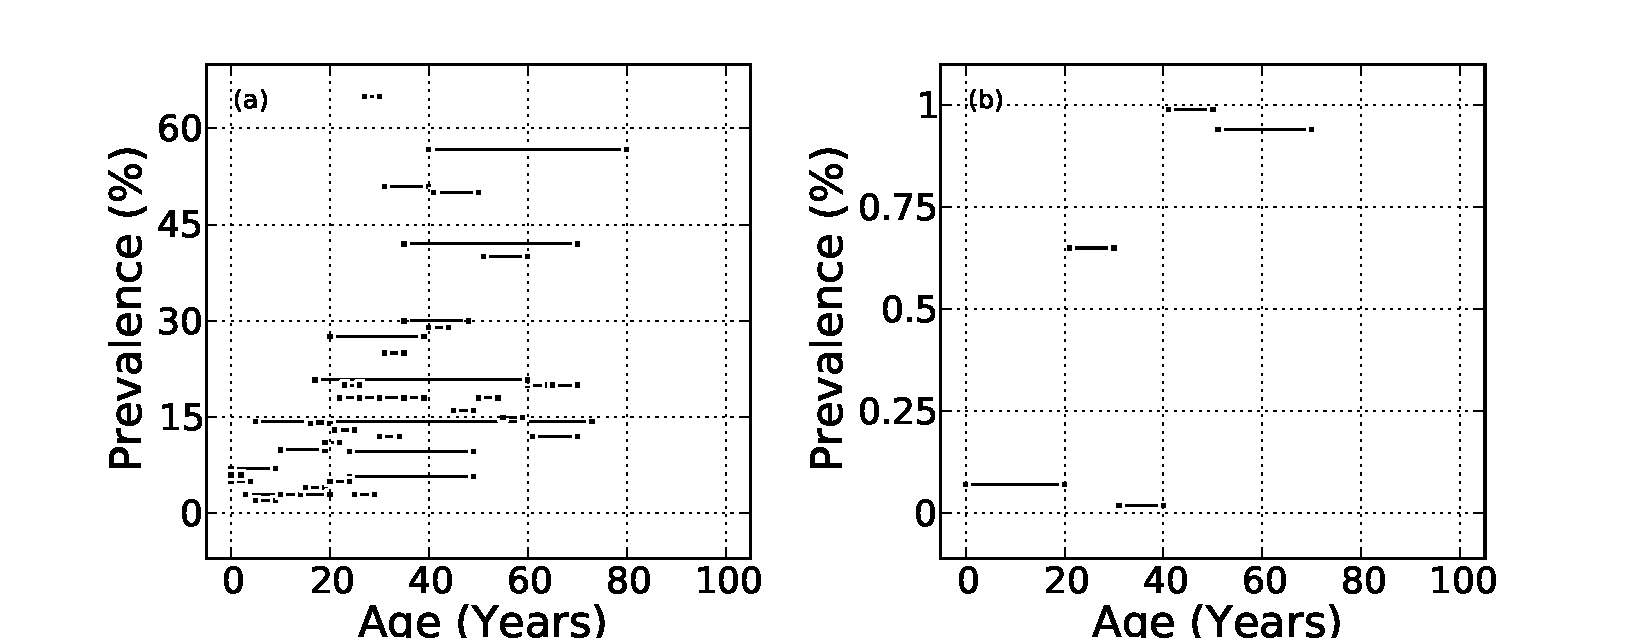
\includegraphics[width=\textwidth]{hepc-EGY_v_JOR.pdf}
            \caption{Prevalence data from systematic review of
              hepatitis C in (a) Egypt and (b) Jordan.}
            \label{fig:app-hepc data}
        \end{center}
    \end{figure}

We used the age-standardizing generalized negative binomial spline
model with hierarchical random effects to estimate prevalence.  The
hierarchical random effects allow the model to capture variation
within the region of North Africa and the Middle East.  Looking at
Table \ref{tab:app-hepc regional rfx}, Egypt (EGY) has significantly
higher prevalence than the other countries in the region.  Figure
\ref{fig:app-hepc regional rfx} confirms this as the prevalence
estimate for Egypt is much above the regional average.

    \begin{table}[h]
        \begin{center}
        \begin{tabular}{|c|c|c|c|}
            \hline
                Country & Posterior Mean & Lower 95\% HPD  & Upper 95\%  HPD \\
            \hline
                EGY	&	1.88	&	 1.6	&	2.2	\\
                JOR	&	-0.59	&	-1.1	&	-0.2 \\
                SAU	&	-0.78	&	-1.1	&	-0.4 \\
                IRQ	&	0.07	&	-0.4	&	0.6	\\
                IRN	&	0.00	&	-0.5	&	0.4	\\
                YEM	&	0.04	&	-0.3	&	0.4	\\
                TUR	&	-0.32	&	-0.7	&	0.0	\\
                SYR	&	-0.16	&	-0.6	&	0.4	\\
                TUN	&	-0.19	&	-0.7	&	0.3	\\
            \hline
        \end{tabular}
        \end{center}
        \caption{ Estimates of the country-level random effect for HCV
          prevalence (an intercept shift in log space) from the random
          effects model for the countries in the North Africa/Middle
          East region.}
        \label{tab:app-hepc regional rfx}
    \end{table}

    \begin{figure}[h]
        \begin{center}
            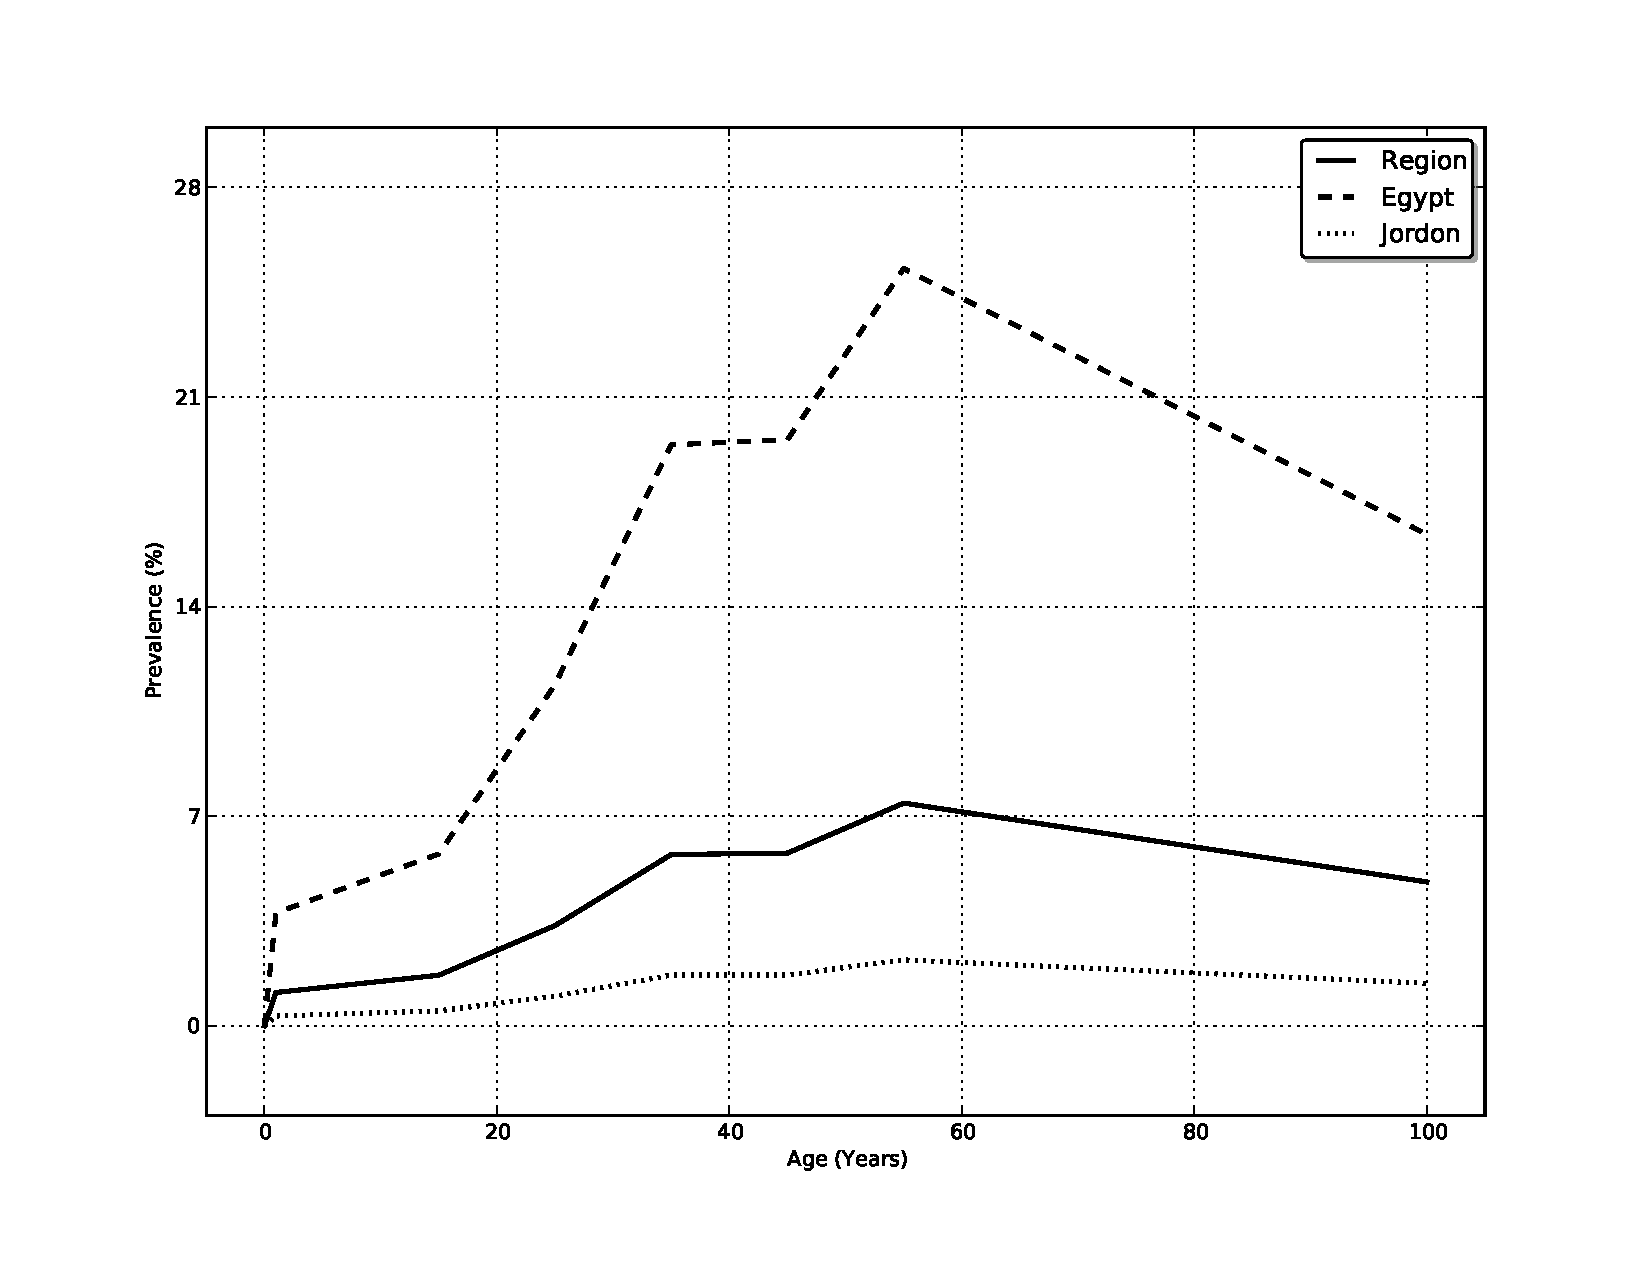
\includegraphics[width=\textwidth]{hepc-region_v_EGY_v_JOR.pdf}
            \caption{The 1990 estimate of hepatitis C prevalence for
              men in the region of North Africa and Middle East and
              the countries Egypt and Jordan.  These estimates only
              use $2$ levels in the hierarchal random effects
              model, region and country.}
            \label{fig:app-hepc regional rfx}
        \end{center}
    \end{figure}

In addition to hierarchical random effects, the negative binomial
rate model includes a parameter that estimates
the amount of nonsampling error, parameterized as the overdispersion
term, $\delta$, described in Chapter~\ref{theory-rate_model}.
In such noisy data, weakly informative priors on $\delta$ help with
convergence and inform the posterior estimates about beliefs
regarding data heterogeneity.  This allows the model to incorporate
expert beliefs about how much of the country-to-country variation is
true variation and how much is nonsampling error, which can be
important in the presence of sparse and noisy data.  We compared three
alternative priors on the negative binomial model dispersion
parameter, $\delta$, corresponding to `very', `moderately' or
`slightly' overdispersed.  The natural logarithm of $\delta$ is
uniformly distributed between its lower and upper bounds.  Intended as
a weakly informative prior, the bounds of the categories overlap, so
that the bounds of `very', `moderately' and `slightly' are $[1,9]$, $[3,27]$ and
$[9,81]$, respectively.

In this example, the effects of priors on the overdispersion of
$\delta$ are seen in the posterior estimates at the country level as
seen in Figure \ref{fig:app-hepc global hetero}.  Random effects
modeling detects within sample variation and true variation that
cannot be explained by a covariate.  Therefore, a change in the prior
on global heterogeneity changes the level of variation and thus the
random effect size.  As seen in Figure \ref{fig:app-hepc global
  hetero}, when the prior on overdispersion is `very', the estimates
are compressed, as compared to a prior of `slightly' overdispersed.

    \begin{figure}[h]
        \begin{center}
            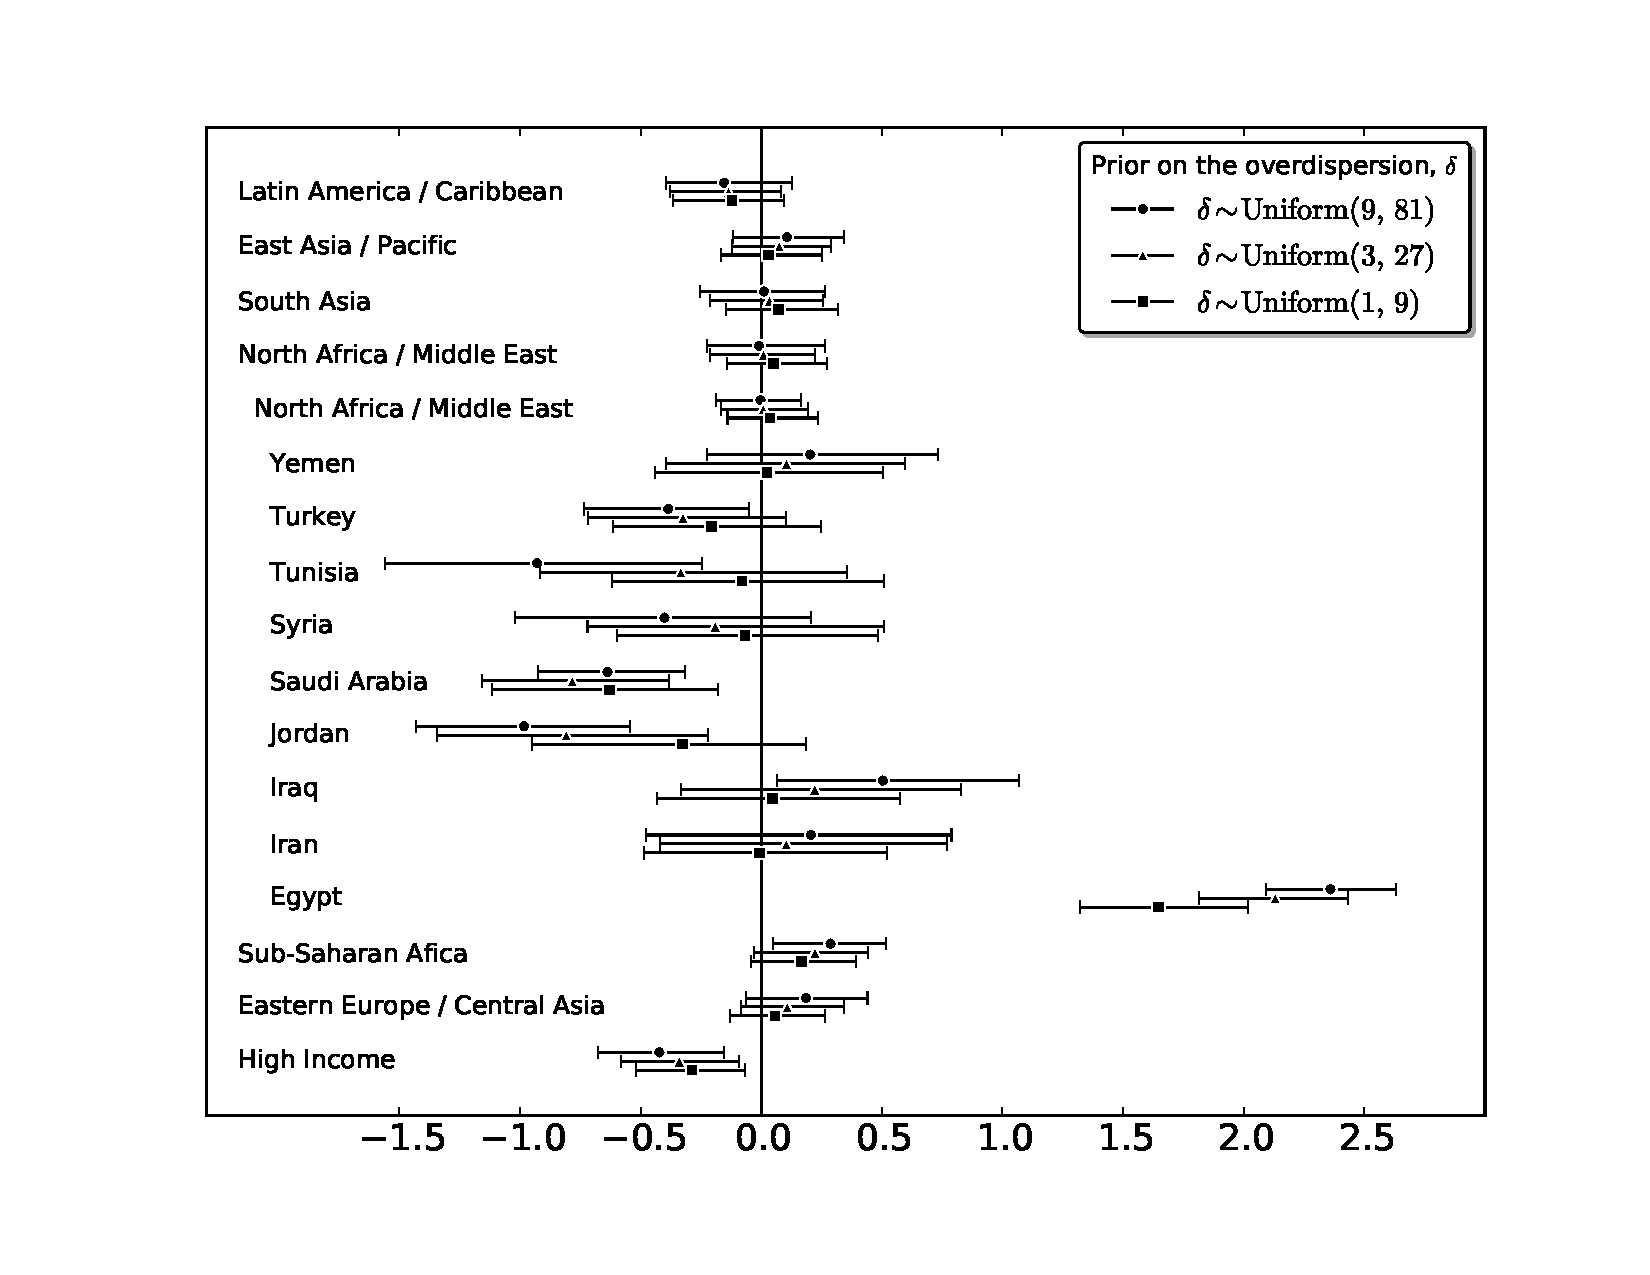
\includegraphics[width=\textwidth]{hepc-tree_plot_global_hetero.pdf}
            \caption{The 1990 intercept shift of hepatitis C
              prevalence in log space for men with different priors on
              global heterogeneity, $\delta$.  Four levels (global,
              super-region, region, country) were used in the
              hierarchal random effects spline model.}
            \label{fig:app-hepc global hetero}
        \end{center}
    \end{figure}

Another way to view compressed estimates is by looking at the
age-standardized prevalence in Table \ref{tab:app-hepc global rfx}.
As heterogeneity increases from `slightly' to `very', country
estimates are compressed toward the regional mean.

    \begin{table}[h]
        \begin{center}
        \begin{tabular}{|c|c|c|c|}
            \hline
                & & Posterior & Standard \\
                Geographic Area & Heterogeneity & Mean & Deviation \\
            \hline
                & $\delta \sim \Uniform(9,81)$ & 0.048 & 0.003 \\
                North Africa Middle East & $\delta \sim \Uniform(3,27)$ & 0.049 & 0.004 \\
                & $\delta \sim \Uniform(1,9)$ & 0.045 & 0.005 \\
            \hline
                & $\delta \sim \Uniform(9,81)$ & 0.007 & 0.002 \\
                Jordan & $\delta \sim \Uniform(3,27)$ & 0.010 & 0.003 \\
                & $\delta \sim \Uniform(1,9)$ & 0.020 & 0.006 \\
            \hline
                & $\delta \sim \Uniform(9,81)$ & 0.188 & 0.012 \\
                Egypt & $\delta \sim \Uniform(3,27)$ & 0.178 & 0.017 \\
                & $\delta \sim \Uniform(1,9)$ & 0.136 & 0.019 \\
            \hline
        \end{tabular}
        \end{center}
        \caption{ Hepatitis C age-standardized prevalence estimates
          from a hierarchal random effects spline model with differing
          priors on global heterogeneity.}
        \label{tab:app-hepc global rfx}
    \end{table}

Hierarchical random effects and the overdispersion parameter, $\delta$,
allow the model to distinguish between true country-to-country variation
and nonsampling error.  Weakly informative priors on $\delta$ incorporate
modeler's beliefs about data heterogenity while the hierarchical random
effects provide a way to model regional variation.  TK concluding sentence.

